\chapter{Electroweak and QCD physics at LHC}\label{chap1}
\thispagestyle{empty}

In this chapter the Standard Model of particle physics is briefly described, in particular the main characteristics of the electroweak and strong interactions are discussed, as well as the machanism of the electroweak symmetry breaking.
In addition, the phenomenology of the proton-proton interactions is described and the main features of the Monte Carlo simulation techniques are given.
Eventually, an overview of the Higgs boson physics from an experimental point of view is reported.

\section{The Standard Model of particle physics}
%%%%%%%%%%%%%%%%%%%%%%%%%%%%%%%%%%%%%%%%%%%%%%%%%%%%%%%%%%%%%%%%%%%%%%
\label{sec:SM}

The Standard Model of Particle Physics is the theory that describes all fundamental constituents of matter and their interactions~\cite{Halzen:1984mc}. It is a renormalisable quantum field theory based on a $\mathrm{SU(3)_c \otimes SU(2)_L \otimes U(1)_Y}$ local gauge symmetry, and is capable to provide a quantitative description of three of the four interactions in nature: electromagnetism, weak interaction and strong nuclear force. 

According to the SM, the ordinary matter is made up of spin-$1/2$ particles, denoted as fermions. The fermions are subdivided into two classifications of elementary particles: leptons and quarks. Both classes consist of six particles, grouped into three doublets, called generations. Additional three doublets for each class are composed of leptons and quarks antiparticles. A charged particle with electric charge $Q=-1$, either the electron e, the muon $\mu$ or the tauon $\tau$, and a neutral particle, the corresponding neutrino, compose the following lepton generations, ordered according to an increasing mass hierarchy:

\begin{equation}
\label{eq:leptons}
\begin{pmatrix} \rm e^-       \\ \nu_{\rm e}      \end{pmatrix}, \quad
\begin{pmatrix} \mu^-     \\ \nu_{\mu}  \end{pmatrix}, \quad
\begin{pmatrix} \tau^-    \\ \nu_{\tau} \end{pmatrix}  \quad .
\end{equation}

Charged leptons can interact via the electromagnetic and weak force, while neutrinos, that are assumed to be massless, can interact only through the weak interaction.

Similarly, the quarks are organized in pairs composed of a particle with $Q=+2/3$, \emph{up} (u), \emph{charm} (c) and \emph{top} (t) quarks, and another particle with $Q=-1/3$, \emph{down} (d), \emph{strange} (s) and \emph{bottom} (b) quarks:

\begin{equation}
\label{eq:quarks}
\begin{pmatrix} \rm u       \\ \rm d      \end{pmatrix}, \quad
\begin{pmatrix} \rm c       \\ \rm s      \end{pmatrix}, \quad
\begin{pmatrix} \rm t       \\ \rm b      \end{pmatrix}  \quad .
\end{equation}

As well as leptons, quarks can interact via the electromagnetic and weak force, but also through the strong interaction, responsible of their confinement within hadrons. In fact, free quarks are not observed in nature, but they bind together forming two categories of hadrons: mesons, bound states of a quark q and an anti-quark $\mathrm{\bar{q}}$, and baryons, bound states of three quarks.

In the SM the interaction between elementary particles occurs through the exchange of spin-1 particles, known as bosons, which identify the fundamental forces. The photon $\gamma$ is the mediator of the electromagnetic interaction, the $\mathrm{W^{\pm}}$ and Z bosons are the mediators of the weak interaction, while the strong force is mediated by eight gluons g. Electromagnetic and weak interactions are actually the manifestations of the same fundamental interaction, the electroweak force.


%%% EWK
\subsection{The electroweak interaction}

The theory of electroweak interaction was formulated in the 1960s by S. L. Glashow, A. Salam and S. Weinberg~\cite{Glashow:1961tr,Weinberg:1967tq} as an $\mathrm{SU(2) \otimes U(1)}$ local gauge theory.
The Lagrangian density governing the electroweak interaction is therefore invariant under gauge transformations of the $\mathrm{SU(2)_L\otimes U(1)_Y}$ symmetry group. The $\mathrm{SU(2)_L}$ group refers to the weak isospin charge $I$, while $\mathrm{U(1)_Y}$ to the weak hypercharge $Y$, which are connected to the charge Q by the following equation:

\begin{equation}
Y = 2(Q - I_3) \quad,
\end{equation}

\noindent where $I_3$ represents the third component of the weak isospin. 

According to the Noether theorem, the $\mathrm{SU(2)_L}$ invariance of the theory leads to the existence of three conserved currents, $J_\mu^\pm$ and $J_\mu^3$, which constitute an isospin triplet of weak currents. 
The two currents $J_\mu^\pm$ represent the weak charged current interactions, which describe the interaction between fermions that are mediated by the charged $\mathrm{W^\pm}$ bosons. These currents only involve left-handed particles or right-handed anti-particles, in accordance with the fact that the parity symmetry is maximally violated for weak charged current interactions, as confirmed by the experiments of Madame Wu~\cite{Wu:1957my} and Garwin-Lederman-Weinrich~\cite{Garwin:1957hc} in 1957. In the case of leptons, charged currents can only connect two particles within the same generation, for example the electron and the electron neutrino, while for the quarks a mixing of different generations may occur, according to the Cabibbo-Kobayashi-Maskawa matrix (CKM).

Another possible interaction in the weak sector is known as neutral current interaction and is mediated by the neutral Z boson. In the vertex of this interaction the identity of the interacting lepton does not change, resembling in this matter the electromagnetic current. Concerning the quark sector, the weak neutral currents involving different quark flavours, i.e. \emph{flavour changing neutral currents}, are strictly suppressed at tree level by the Glashow-Iliopoulos-Maiani mechanism (GIM)~\cite{Glashow:1970gm}.

Nevertheless, the other component of the weak isospin triplet of currents $J_\mu^3$, cannot be identified with the weak neutral current, because the weak neutral current involves both left- and right-handed components. The electromagnetic current cannot be represented by $J_\mu^3$ as well, for the aforementioned reason and because it cannot be coupled with the uncharged neutrino. In order to save the $\mathrm{SU(2)}$ symmetry, the existence of the $\mathrm{U(1)_Y}$ symmetry is required, and a new conserved current, $j_\mu^Y$, arises. The $j_\mu^Y$ current is unchanged under $\mathrm{SU(2)}_L$ transformations (is an isospin singlet) and is incorporated, together with $J_\mu^3$, in the definition of the electromagnetic current, giving rise to the electroweak unification.

Local gauge symmetries naturally lead to the presence of gauge bosons, the exchange particles mediators of the fundamental interactions. The symmetry requires these gauge bosons to be massless, which is unproblematic for photons and gluons, but in drastic contrast to the known masses of the Z and $\mathrm{W^\pm}$ bosons, which are $m_\mathrm{Z} = 91.1876 \pm 0.0021$\GeV and $m_\mathrm{W} = 80.385 \pm 0.015$\GeV, respectively. Moreover, the maximally parity violating structure of the weak charged currents also breaks local gauge invariance for all massive fermions, due to their coupling to the W boson. This leads to the apparent antagonism that, while the $\mathrm{SU(2)_L \otimes U(1)_Y}$ gauge symmetry does describe the coupling structure of the electroweak force, at the same time it seems to contradict the fact that the W and Z bosons, and all fermions have a non-vanishing mass. 

The proposed solution to this problem is the mechanism of \emph{spontaneous symmetry breaking}, where the gauge symmetry is still intrinsic to the Lagrangian density of the theory, but not manifest in its energy ground state, which in this case is the quantum vacuum. The spontaneous symmetry breaking of the $\mathrm{SU(2)_L \otimes U(1)_Y}$ symmetry group requires the introduction of a self-interacting complex scalar field~\cite{Wolf:2015kua}, which is an isospin doublet:
\begin{equation}
\phi = \begin{pmatrix} \phi^+       \\ \phi^0      \end{pmatrix} = \begin{pmatrix} (\phi_1+i\phi_2)/\sqrt{2}       \\ (\phi_3+i\phi_4)/\sqrt{2}      \end{pmatrix} \quad .
\end{equation}

\noindent The simplest lagrangian involving this field has the form:
\begin{equation}\label{eq:higgsL}
\begin{split}
\mathcal{L}_\mathrm{H} &= \mathcal{D}_\mu \phi^\dagger \mathcal{D}^\mu \phi - V(\phi) \quad,\\
V(\phi) &= -\mu^2\phi^\dagger\phi + \lambda(\phi^\dagger\phi)^2
\end{split}
\end{equation}

\noindent Here th $\mathcal{D}_\mu$ represents the covariant derivative defined as:
\begin{equation}
\mathcal{D}_\mu = \partial_\mu + i g \vec{A}_\mu \cdot \frac{\vec{\tau}}{2} - \frac{1}{2}i g' Y B_\mu \quad ,
\end{equation}
\noindent where $\vec{A}_\mu$ is a vector of three gauge fields satisfying the local $\mathrm{SU(2)}$ symmetry, and $B_\mu$ is the gauge field assuring the $\mathrm{U(1)}$ symmetry. The parameters $g$ and $g'$ represent the coupling constants for the gauge fields.

The term $V(\phi)$ in Eq.\eqref{eq:higgsL} is a potential term that depends on two parameters, $\mu$ and $\lambda$, with $\lambda>0$ in order to have vacuum stability. If the $\mu$ parameter is chosen so that $\mu^2<0$, the symmetry of $V(\phi)$ may be broken, since its minimum value is degenerate:
\begin{equation}
\phi^\dagger\phi = -\frac{\mu^2}{2\lambda} = \frac{v^2}{2} \quad ,
\end{equation}

\noindent where $v$ corresponds to the \emph{vacuum expectation value} (VEV). Perturbation theory requires an expansion of $\phi$ around its energy ground state. The ground state is chosen in such a way it  breaks the $\mathrm{SU(2)_L \otimes U(1)_Y}$ symmetry group but preserves the invariance under $\mathrm{U(1)_{em}}$ transformations, i.e. it has a null electric charge. This latter requirement guarantees the presence of a neutral massless gauge boson, the photon. Therefore, the ground state can be written without any loss of generality as:
\begin{equation}
\tilde{\phi} = \frac{1}{\sqrt{2}} \begin{pmatrix} 0 \\ v   \end{pmatrix}\quad .
\end{equation}
The field $\phi$ can be expanded at first order around the ground state obtaining:
\begin{equation}
\phi = \frac{1}{\sqrt{2}} \begin{pmatrix} 0 \\ v+h   \end{pmatrix}\quad .
\end{equation}
Introducing this field in the Higgs Lagrangian in Eq.~\eqref{eq:higgsL}, the bosonic fields acquire a mass given by:
\begin{equation}
m_\mathrm{W} = \frac{v}{2}g \qquad m_\mathrm{Z} = \frac{v}{2}\sqrt{g^2 +g'^2} \quad,
\end{equation}
\noindent where $g$ and $g'$ are the electroweak coupling constants for the gauge fields.

Furthermore, given the self-interaction terms of the $h$ field, a new physical state also arises (the Higgs boson) with a mass:
\begin{equation}
m_\mathrm{H} = v\sqrt{2\lambda} \quad.
\end{equation}
\noindent whose value is not predicted by the theory, since $\lambda$ is unknown\footnote{On the other hand, the value of $v$ can be obtained using the relation between $m_\mathrm{W}$ and the Fermi constant $G_\mathrm{F}$, which leads to $v = 1/\sqrt{\sqrt{2}G_\mathrm{F}} = 246.22$\GeV, setting the scale of the electroweak symmetry breaking.}.

The mass of fermions is achieved without breaking the gauge symmetry of the Lagrangian by introducing a coupling term, known as Yukawa coupling, between the fermion doublets and the Higgs field.

In addition to the mass of the particles, the model also predicts the couplings $f$ of the Higgs boson to fermions and heavy gauge bosons, despite their numerical values need to be determined by experiments:
\begin{equation}
\begin{split}
f_\mathrm{H\to ff} &\propto \frac{m_\mathrm{f}}{v} ,\quad \text{fermions}\\
f_\mathrm{H\to VV} &\propto \frac{2m_\mathrm{V}^2}{v} ,\quad \text{heavy bosons trilinear}\\
f_\mathrm{HH\to VV} &\propto \frac{2m_\mathrm{V}^2}{v^2} ,\quad \text{heavy bosons quartic}\\
f_\mathrm{H\to HH} &\propto \frac{3m_\mathrm{H}^2}{v} ,\quad \text{Higgs boson trilinear}\\
f_\mathrm{HH\to HH} &\propto \frac{3m_\mathrm{H}^2}{v^2} ,\quad \text{Higgs boson quartic} \quad .
\end{split}
\end{equation}

During the past decades the predictions of the SM have been confirmed by experimental results with outstanding precision, and in 2012 the discovery of a new boson with a mass of about 125\GeV, consistent with the predicted Higgs boson, was announced by the ATLAS and CMS experiments at LHC.


\subsection{The strong interaction}

Quantum Chromo-Dynamics (QCD) is the theory that describes the strong interactions~\cite{Ellis:1991qj}. It is an unbroken gauge non-abelian theory based on the group $\mathrm{SU(3)}$ of colour ($\mathrm{SU(3)_c}$). The mediators of the interaction are eight massless gluons and the elementary particles of matter are colour triplets of quarks, with different flavours. In fact, as shown in \eqref{eq:quarks}, six types (flavours) of quark exist and each quark possesses a colour charge that can assume three values, namely red, green and blue.

The physical vertices in QCD include the gluon-quark-antiquark vertex, analogous to the Quantum Electro-Dynamics (QED) photon-fermion-antifermion coupling, but also the three-gluon and four-gluon vertices, i.e. gluon themselves carry colour charge, which have no analogue in an abelian theory like QED. Quark and gluons are the only particles that interact through the strong interaction.

The non-abelian nature of the theory leads to two important characteristics:
\begin{itemize}
\item \emph{colour confinement}: the QCD coupling constant $\alpha_s = g_s^2/4\pi$ is a function of the scale of the interaction $Q$. At low energy (corresponding to large distances of the order of 1\,fm) the $\alpha_s$ value is large and a perturbative approach is not applicable. When a quark-antiquark pair begins to separate, the colour field generated by the exchanged gluons increases its intensity and, at some point, the creation of a new quark-antiquark pair from the vacuum becomes more energetically favourable than increasing further the interaction strength. This explains why free quarks are not observed and the final state particles are made of colourless quark bound states (hadrons). This is also the cause of the hadronization process which causes the formation of jets.

\item \emph{asymptotic freedom}: the coupling constant decreases at large scales $Q$ approaching to zero, meaning that quarks can be asymptotically considered as free particles. The small value of the coupling constant at large scales justifies the usage of a perturbative approach to describe hard processes.
\end{itemize}


%\section{Electroweak interaction}
%%%%%%%%%%%%%%%%%%%%%%%%%%%%%%%%%%%%%%%%%%%%%%%%%%%%%%%%%%%%%%%%%%%%%%
\label{sec:EW}

The theory of electroweak interaction was formulated in the 1960s by S. L. Glashow, A. Salam and S. Weinberg~\cite{Glashow:1961tr,Weinberg:1967tq} as an $\mathrm{SU(2) \otimes U(1)}$ local gauge theory.
In 1957 the experiments lead by Madame Wu~\cite{Wu:1957my} and Garwin-Lederman-Weinrich~\cite{Garwin:1957hc} confirmed that the parity symmetry is maximally violated for weak charged current interactions, proving that only left-handed particles or right-handed antiparticles are involved in these interactions. 

To express this aspect the weak charged currents can be written making use of the Dirac spinors, $\ell$ and $\nu_\ell$ (representing the lepton and neutrino spinors, repsectively), as follows:

\begin{equation}
\begin{split}
J_\mu^+ &= \bar{\nu}_\ell \gamma_\mu \dfrac{1}{2}(1-\gamma^5) \ell \quad, \\
J_\mu^- &= \bar{\ell} \gamma_\mu \dfrac{1}{2}(1-\gamma^5)\nu_\ell \quad,
\end{split}
\end{equation}

where the ``$+$'' and ``$-$'' superscripts indicate the charge-raising and charge-lowering character of the currents, and $\gamma^5 = i\gamma^0\gamma^1\gamma^2\gamma^3$ is the product of the Dirac $\gamma$ matrices. In fact, the effect of the projector $P=\dfrac{1}{2}(1-\gamma^5)$ is to project the spinor to its left-handed component. Therefore, introducing the following doublet:

\begin{equation}
\chi_L = \begin{pmatrix} \nu_\ell \\ \ell \end{pmatrix}_L \quad ,
\end{equation}

where $L$ denotes the left-handed component of the spinor, and defining the ``step-up'' and ``step-down'' operators $\tau_\pm = \dfrac{1}{2}(\tau_1 \pm i\tau_2)$, where $\tau_i$ are the Puali matrices, the charged currents become:

\begin{equation}
\begin{split}
J_\mu^+ &= \bar{\chi}_L \gamma_\mu \tau_+ \chi_L \quad, \\
J_\mu^- &= \bar{\chi}_L \gamma_\mu \tau_- \chi_L \quad.
\end{split}
\end{equation}

In order to complete the $\mathrm{SU(2)}$ invariance of the theory, a third conserved current should exist with the form:

\begin{equation}
J_\mu^3 = bar{\chi}_L \gamma_\mu \dfrac{1}{2} \tau_3 \chi_L = \dfrac{1}{2}\bar{\nu}_L \gamma_\mu \nu_L -  \dfrac{1}{2}\bar{\ell}_L \gamma_\mu \ell_L \quad,
\end{equation}

The three currents $J_\mu^\pm$ and $J_\mu^3$ constitute an isospin triplet of weak currents, with corresponding charges

\begin{equation}
T^i = \int J_0^i(x)d^3x \quad,
\end{equation}

that generate the $\mathrm{SU(2)}_L$ algebra defined by the following rules:

\begin{equation}
\left[T^i, T^j \right] = i \varepsilon_{ijk} T^k \quad.
\end{equation}

Nevertheless, $J_\mu^3$ cannot be identified with the weak neutral current, because the weak neutral current involves both left- and right-handed components. The electromagnetic current cannot be represented by $J_\mu^3$ as well, for the aforementioned reasons and because it cannot be coupled with the uncharged neutrino.

In order to save the $\mathrm{SU(2)}$ symmetry, the existence of a new $\mathrm{U(1)}$ symmetry is required, and a new conserved current arises. The new symmetry is known as hypercharge symmetry ($\mathrm{U(1)_Y}$) and the corresponding conserved current is:

\begin{equation}
j_\mu^Y = \bar{\psi} \gamma_\mu Y \psi \quad,
\end{equation}

where $\psi$ is a generic Dirac spinor and the hypercharge $Y$ is defined as:

\begin{equation}
Y = 2(Q - T_3)
\end{equation}

The $j_\mu^Y$ current is unchanged under $\mathrm{SU(2)}_L$ transformations (is an isospin singlet). The electromagnetic and weak interactions can be incorporated defining the electromagnetic current as:

\begin{equation}
j_\mu^{em} = J_\mu^3 + \dfrac{1}{2} j_\mu^Y \quad,
\end{equation}

which represents the electroweak unification. 
\begin{comment}
Also, the weak neutral current $J_\mu^{NC}$ can be written as a combination of $J_\mu^3$ and $j_\mu^{em}$ as follows:

\begin{equation}
J_\mu^{NC} = J_\mu^3 - \sin ^2 \theta_W j_\mu^{em} \quad,
\end{equation}

where $\theta_W$ is the Weinberg angle.
\end{comment}
The electroweak lagrangian can be expressed in a local $\mathrm{SU(2)}_L \otimes \mathrm{U(1)}_Y$ gauge invariant form by introducing the covariant derivatives $\mathcal{D}_\mu$ in place of the ordinary derivatives:

\begin{equation}
\mathcal{D}_\mu = \partial_\mu + i g \vec{A}_\mu \cdot \frac{\vec{\tau}}{2} - \frac{1}{2}i g' Y B_\mu \quad ,
\end{equation}

where $\vec{A}_\mu$ is a vector of three gauge fields satisfying the local $\mathrm{SU(2)}$ symmetry, and $B_\mu$ is the gauge field assuring the $\mathrm{U(1)}$ symmetry. The parameters $g$ and $g'$ represent the coupling constants for the gauge fields. The electroweak lagrangian can thus be written as:

\begin{equation}
\mathcal{L} = \sum_{f} \bar{\psi}i\gamma_\mu\mathcal{D}_\mu\psi = \sum_{f} \bar{\psi}i\gamma_\mu\partial_\mu\psi + \mathcal{L}_int \quad,
\end{equation}

where $\mathcal{L}_int$ represents the interaction terms.

\section{The Higgs mechanism}
%%%%%%%%%%%%%%%%%%%%%%%%%%%%%%%%%%%%%%%%%%%%%%%%%%%%%%%%%%%%%%%%%%%%%%
\label{sec:Higgs}

Local gauge symmetries naturally lead to the presence of gauge bosons, the exchange particles mediators of the fundamental interactions. The symmetry requires these gauge bosons to be massless, which is unproblematic for photons and gluons, but in drastic contrast to the known masses of the Z and $\mathrm{W^\pm}$ bosons, which are $m_\mathrm{Z} = 91.1876 \pm 0.0021$\GeV and $m_\mathrm{W} = 80.385 \pm 0.015$\GeV, respectively. Moreover, the maximally parity violating structure of the weak charged currents also breaks local gauge invariance for all massive fermions, due to their coupling to the W boson. This leads to the apparent antagonism that, while the $\mathrm{SU(2)_L \otimes U(1)_Y$ gauge symmetry does describe the coupling structure of the electroweak force, at the same time it seems to contradict the fact that the W and Z bosons, and all fermions have a non-vanishing mass. 

The proposed solution to this problem is the mechanism of spontaneous symmetry breaking, where the gauge symmetry is still intrinsic to the Lagrangian density of the theory, but not manifest in its energy ground state, which in this case is the quantum vacuum.

\section{The strong interaction}
%%%%%%%%%%%%%%%%%%%%%%%%%%%%%%%%%%%%%%%%%%%%%%%%%%%%%%%%%%%%%%%%%%%%%%
\label{sec:QCD}


\section{Phenomenology of proton proton interactions}
%%%%%%%%%%%%%%%%%%%%%%%%%%%%%%%%%%%%%%%%%%%%%%%%%%%%%%%%%%%%%%%%%%%%%%
\label{sec:ppInt}


\section{Monte Carlo simulations}
%%%%%%%%%%%%%%%%%%%%%%%%%%%%%%%%%%%%%%%%%%%%%%%%%%%%%%%%%%%%%%%%%%%%%%
\label{sec:MC}


\section{Experimental Higgs boson highlights}
%%%%%%%%%%%%%%%%%%%%%%%%%%%%%%%%%%%%%%%%%%%%%%%%%%%%%%%%%%%%%%%%%%%%%%
\label{sec:HiggsExp}

The discovery of the new boson has been followed by a comprehensive set of measurements aimed at establishing the properties of the particle. Latest results reported by both the ATLAS and CMS experiments are consistent with the SM expectations for the Higgs boson. The properties that have been measured are, mainly:

\begin{itemize}
\item the signal strength modifier $\mu = \sigma/\sigma_\mathrm{SM}$, where $\sigma$ is the observed production cross section and $\sigma_\mathrm{SM}$ is the value predicted by the SM for a given mass hypothesis;

\item the couplings to bosons and fermions;

\item the spin and parity;

\item the total decay width of the resonance.
\end{itemize}

Moreover, the combination of the results of the two experiments has recently been performed concerning the mass of the new boson, which is found to be $m_\mathrm{H} = 125.09 \pm 0.21 ~\text{(stat.)} \pm 0.11~\text{(syst.)}$\GeV~\cite{Aad:2015zhl}.

The CMS experiment has investigated the Higgs boson decays to ZZ, WW, $\gamma\gamma$, $\tau\tau$ and $\mathrm{b \bar b}$ using 2011 and 2012 data, and is now looking at the same channels using new data collected at a centre-of-mass energy of 13\TeV. The 8\TeV CMS results of all the channels have been combined and the best-fit signal strength corresponding to the measured mass is found to be $\mu = 1.00 \pm 0.09~\text{(stat.)} ^{+0.08}_{-0.07}~\text{(theo.)} \pm  0.07~\text{(syst.)}$~\cite{Khachatryan:2014jba}, in good agreement with the SM expectation $\mu=1$.
The signal strengths modifiers obtained in different sub-combinations of channels for $m_\mathrm{H}=125$\GeV are shown in Fig.~\ref{fig:signal_strengths}, grouped by production mode tag and decay channel.

\begin{figure}[htb]
\centering
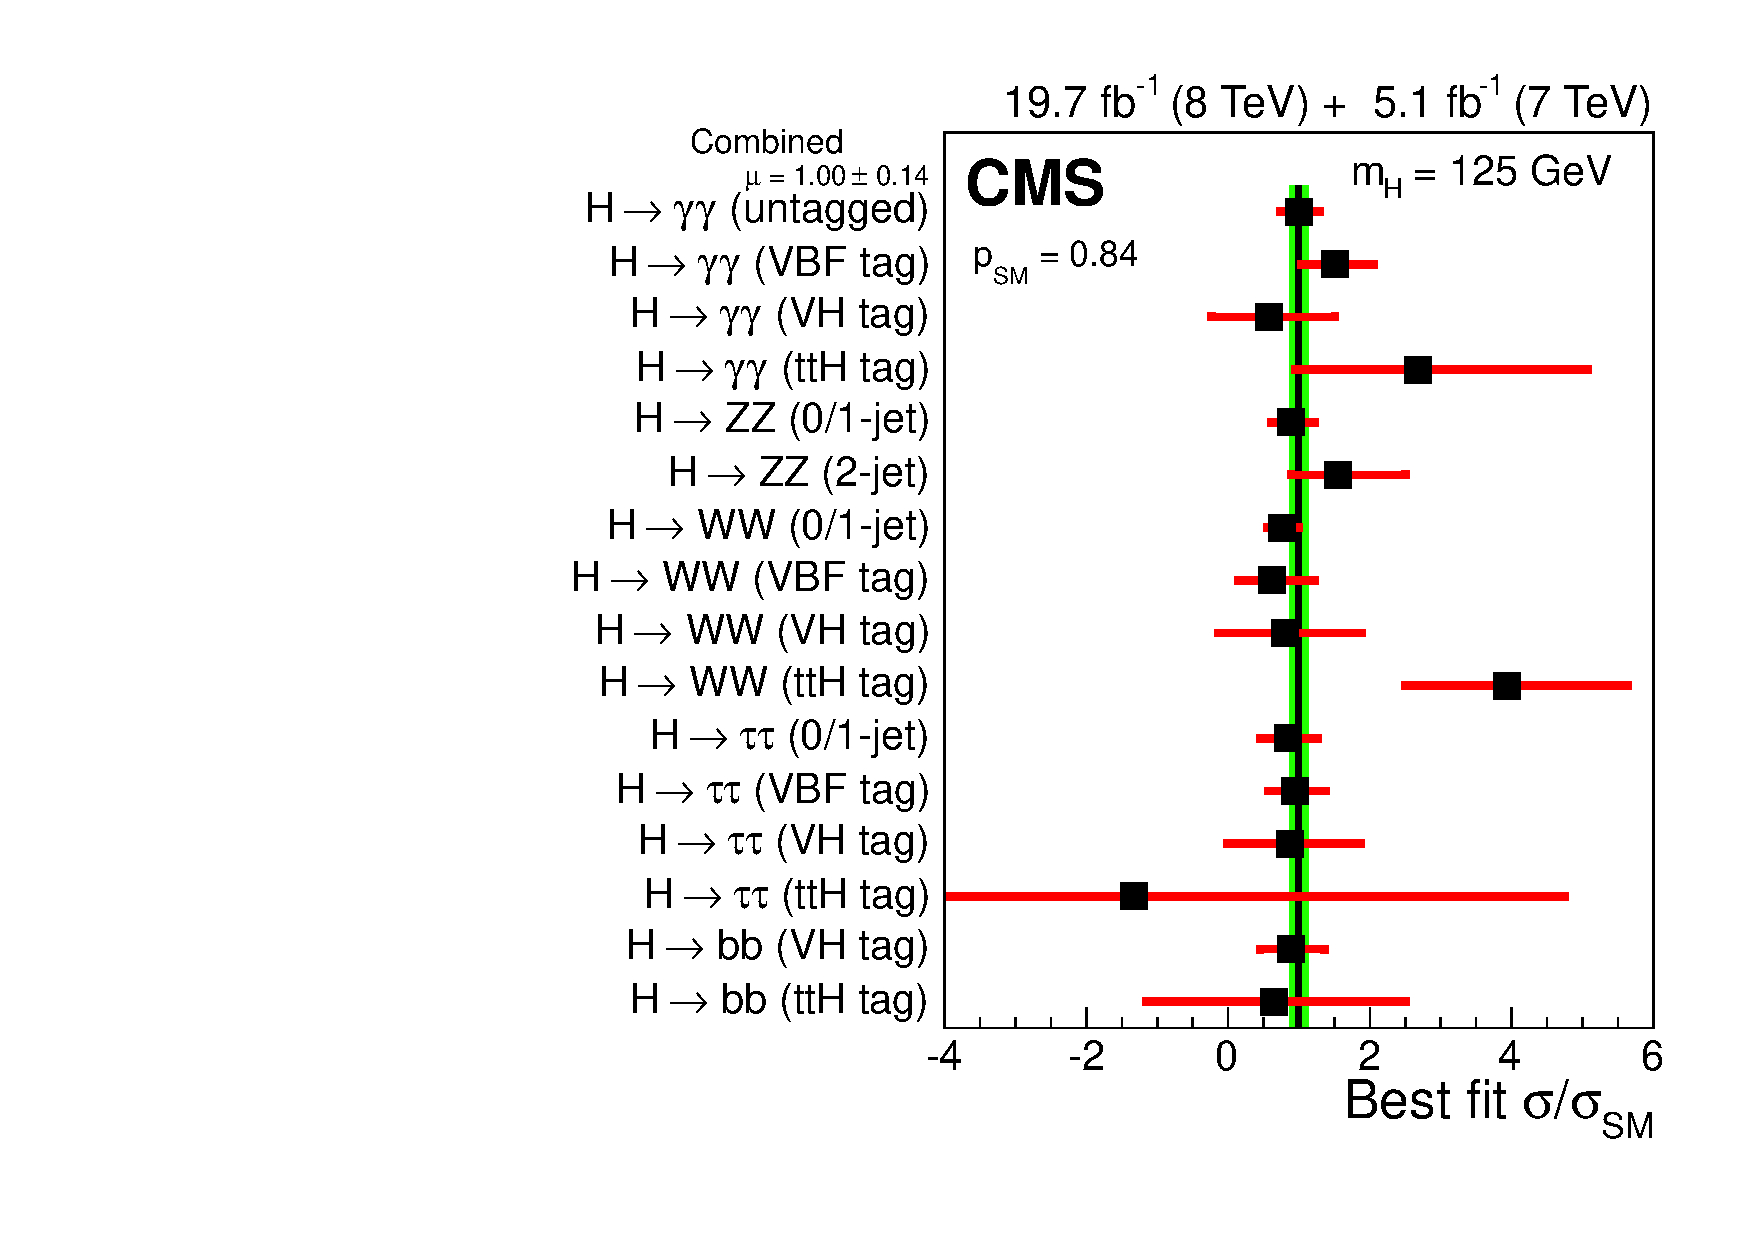
\includegraphics[width=0.7\textwidth]{images/signal_strengths.pdf}
\caption{Values of the best-fit $\mu$ for the overall combined analysis (solid vertical line) and separate combinations grouped by production mode tag and decay channel.}\label{fig:signal_strengths}
\end{figure}
    
The combination of all measurements in all decay channels is used to extract ratios between the observed coupling strengths and those predicted by the SM. The formalism used to test for deviations from the SM expectations has been established by the LHC Higgs Cross Section Working Group in Ref.~\cite{Heinemeyer:2013tqa}. This formalism makes some assumptions, in particular that the observed state has $J^P =0^+$ and that the narrow width approximation holds, leading to a factorization of the coupling strengths for production and decay modes. As an example, Higgs boson events produced via ggH and decaying to WW, i.e. $\mathrm{gg\to H\to WW}$, can be used to measure the Higgs boson coupling to W bosons and to fermions (mainly top quarks due to their presence in the gluon fusion loop). The combination of ATLAS and CMS results using data collected at 7 and 8\TeV is used to test the Higgs boson coupling to fermions $k_F$ and bosons $k_V$~\cite{Khachatryan:2016vau}. The contours at 68\% CL in the $(k_F^f, k_V^f)$ plane (where the $f$ refers to the generic decay channel H$\to f$) for the combination of ATLAS and CMS results and for the individual channels are shown in Fig.~\ref{fig:couplings}.

\begin{figure}[htb]
\centering
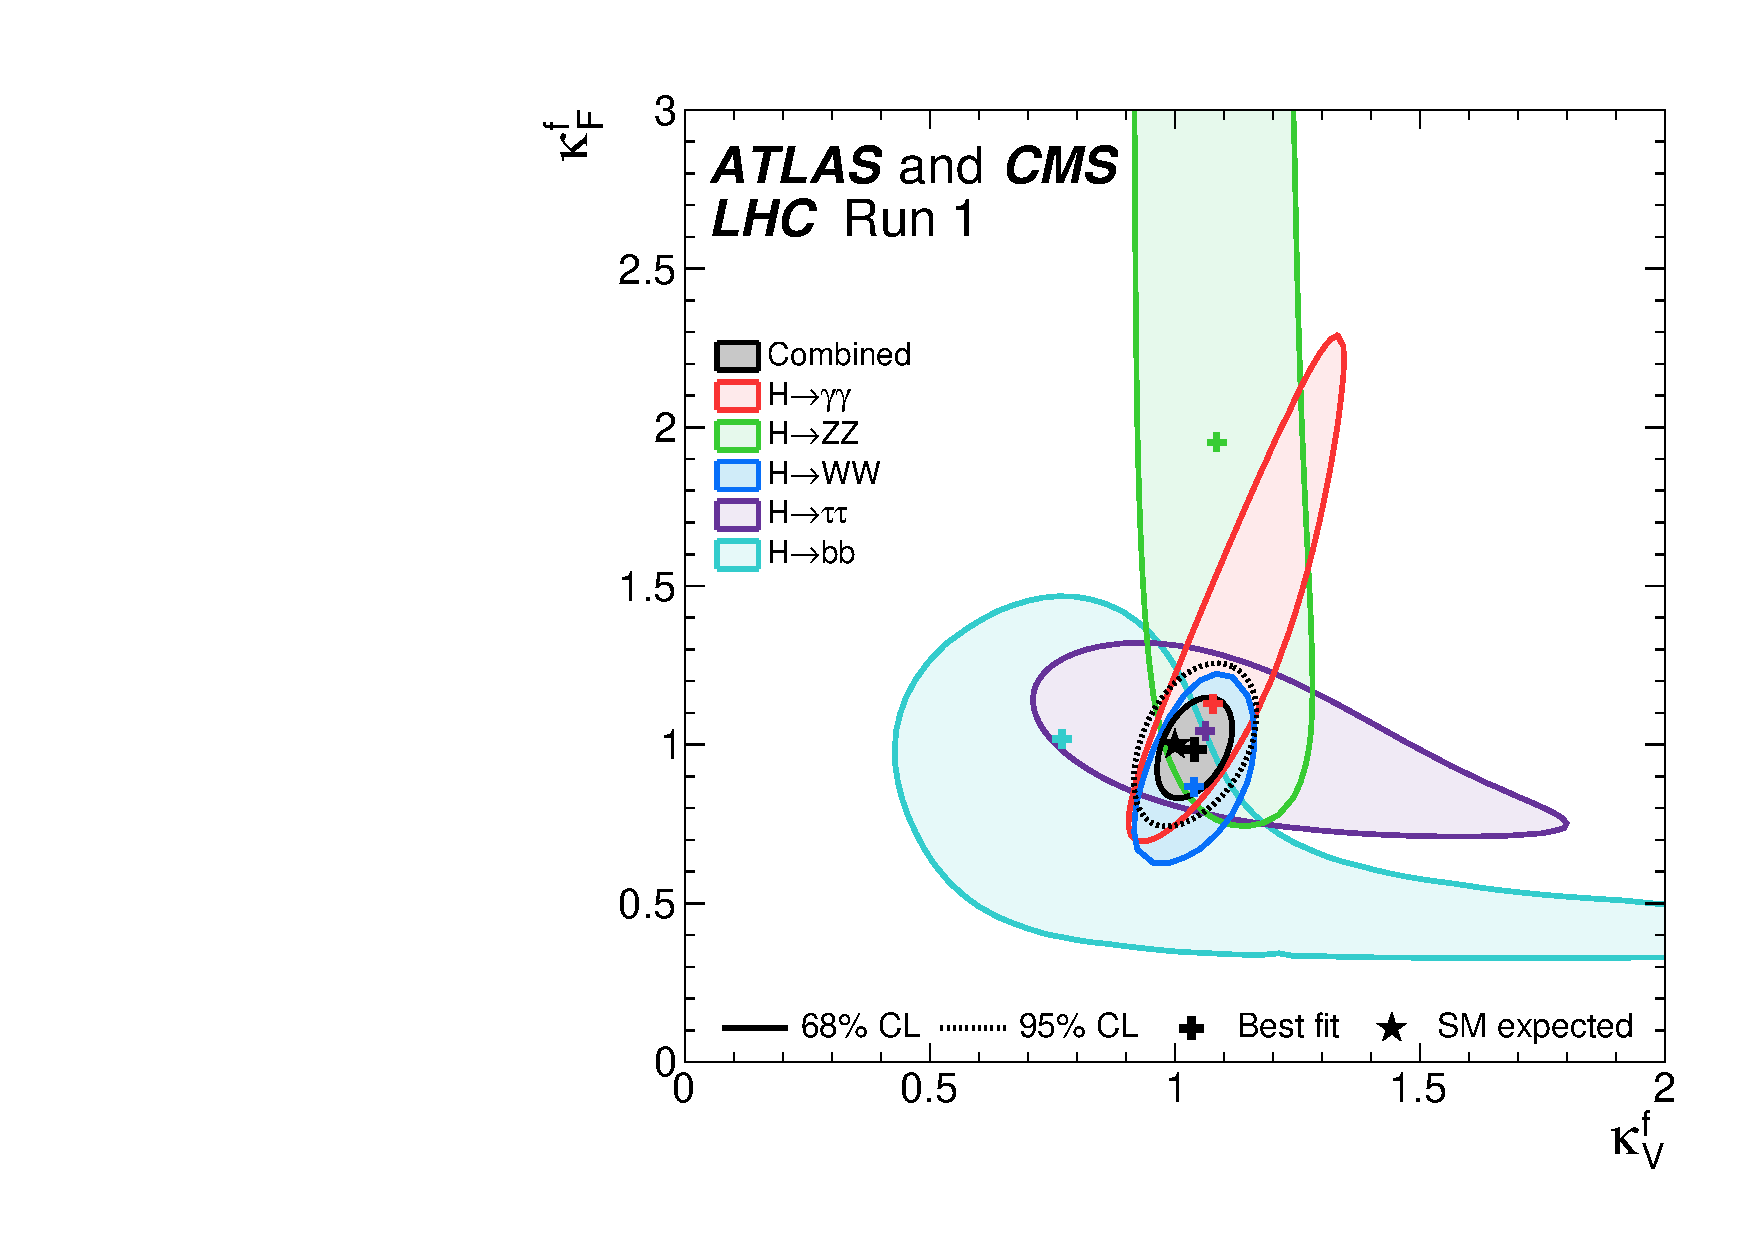
\includegraphics[width=0.7\textwidth]{images/couplings.pdf}
\caption{Contours at 68\% CL in the $(k_F^f, k_V^f)$ plane for the combination of ATLAS and CMS results and for the individual channels.}\label{fig:couplings}
\end{figure}

The combined result is in agreement with the SM expectation and the final confidence interval is driven by the \hww channel, which provides the most precise determination of $k_F^f$ and $k_V^f$ because it is the only channel that provides significant constraints on both parameters through the measurements of the ggH and VBF production processes.

About the spin and parity properties, the results of the H$\to \gamma\gamma$, H$\to$ZZ$\to 4\ell$ and \hwwllnn channels confirmed the hypothesis of a scalar boson ($J^P = 0^+$), excluding the other hypotheses with a confidence level of 99\% or higher.

The Higgs boson total decay width ($\Gamma_\mathrm{H}$) is predicted by the SM as a function of its mass, as shown in Fig.~\ref{fig:width}. At $m_\mathrm{H}=125$\GeV the Higgs boson is predicted to be a narrow resonance, with a total decay width of the order of 4.1\MeV. Direct measurements of the decay width have been performed in the H$\to$ZZ$\to 4\ell$ and H$\to\gamma\gamma$ channels, but the results are limited by the experimental resolution, which is about three orders of magnitude larger than the expected value, thus not allowing to provide significant constraints. The sizeable off-shell production of the Higgs boson can also be used to constrain its natural width. In fact, a measurement of the relative off-shell and on-shell production provides direct information on $\Gamma_\mathrm{H}$~\cite{Caola:2013yja}, under the assumption that the Higgs boson off- and on-shell production mechanisms are the same as in the SM and the ratio of couplings governing the two remains unchanged with respect to the SM predictions. Using this technique and combining the CMS results of the H$\to$ZZ$\to 4\ell$ and \hwwllnn channels, the upper limit at 95\% CL on the Higgs boson total decay width is found to be $\Gamma_\mathrm{H}^\mathrm{obs} < 13$\MeV~\cite{Khachatryan:2016ctc}, which represents a far better constraint with respect to direct measurements.

\begin{figure}[htb]
\centering
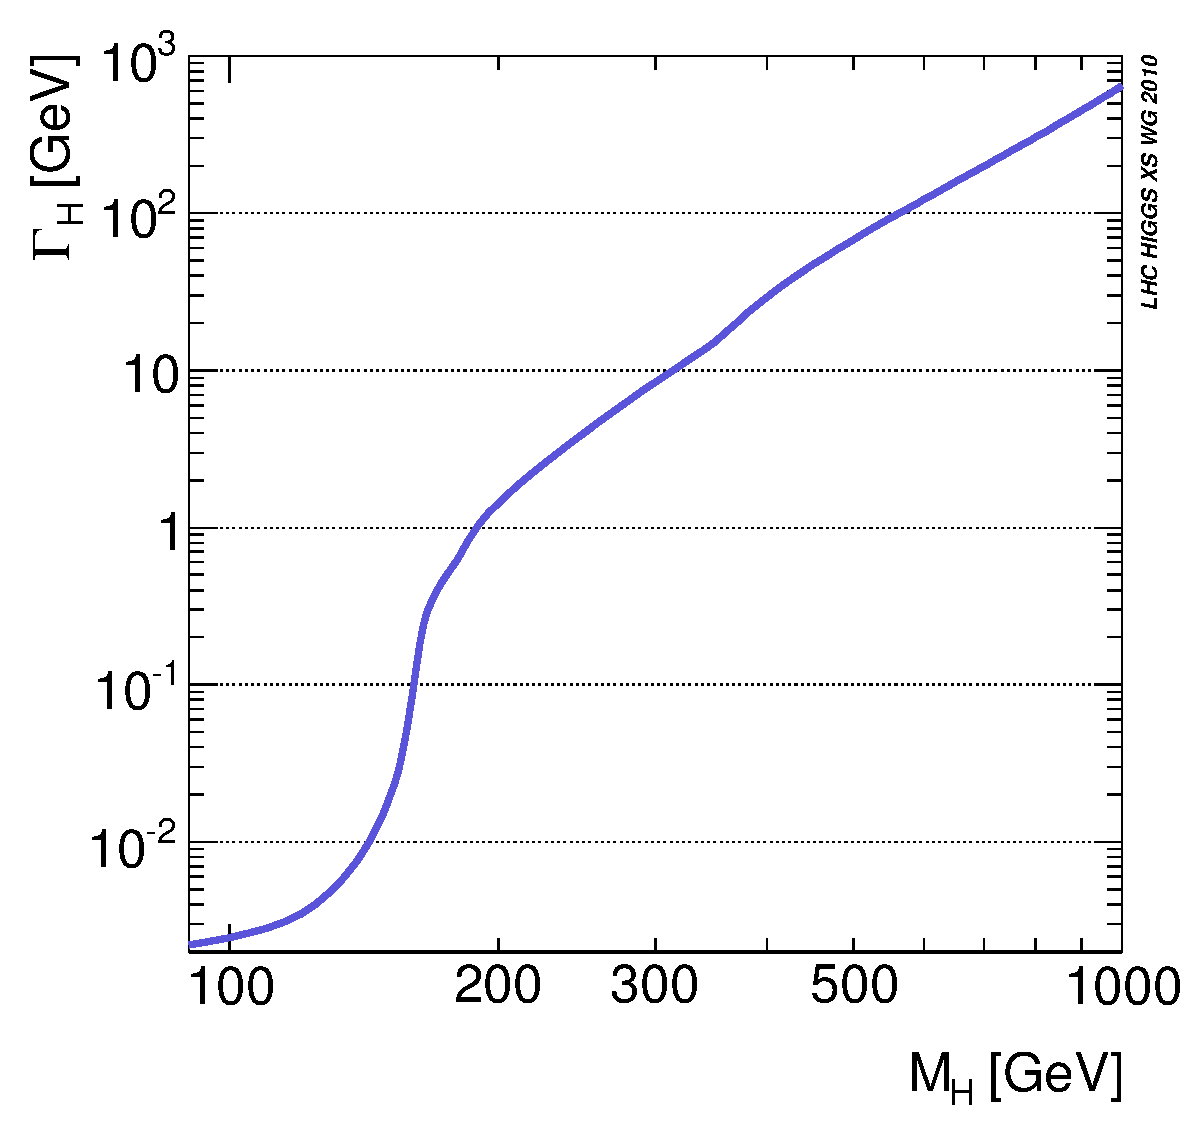
\includegraphics[width=0.7\textwidth]{images/width.pdf}
\caption{Total decay width of the SM Higgs boson as a function of $m_\mathrm{H}$.}\label{fig:width}
\end{figure}

Differential cross section measurements have also been performed by both experiments in the bosonic channels, $\gamma\gamma$, ZZ and $\mathrm{W^+W^-}$ (the latter is presented in Chapter~\ref{chap4} of this work), showing agreement with the SM-based theoretical predictions.

